\section{A numerical sign and scale check}
\label{sec:numerics}

The proof above is analytic.  We nevertheless use the exact chart
\cref{eq:exact-chart} for an independent diagnostic of the sign and scale of
\(c_\perp\).  The computation is deliberately kept separate from the
definition of \(\mathfrak d_\cP\): it prescribes a leading-order history and
uses a finite energy section, so its root is not a complete-history
intersection.

\subsection{Method of steps}

On \([-S-\theta_1,-S]\), prescribe the singular canard
\cref{eq:singular-canard} and the singular transverse graph
\cref{eq:singular-stable-graph}.  Starting at \(-S\), integrate the literal
four-dimensional RFDE \cref{eq:exact-chart} by the method of steps.  Each
step interval is solved with an implicit Radau method, and previous dense
solutions provide history interpolation; see \citet{shampine2001solving}
for the method-of-steps principle.  At \(+S\), tune \(\nu\) with a Brent
root solve until the normalized first integral \cref{eq:first-integral} is
zero.

For a symmetric redistribution step \(h=0.04\), the reported quotient is
\begin{equation}
\label{eq:numerical-quotient}
 q_{\rm num}(\del,S)
 =\frac{\nu_c(\del,h;S)-\nu_c(\del,-h;S)}{2\del h}.
\end{equation}
The theorem predicts
\begin{equation}
\label{eq:numerical-target}
 c_\perp=\frac{K(\theta_0-\theta_1)}{4\alpha}
 =-0.2041241452319315
\end{equation}
for
\(K=1\), \((\theta_0,\theta_1)=(0.5,1)\), and
\(d_w=1.5\).

The central quotient moves toward \cref{eq:numerical-target}; at the
smallest \(\del\), its relative discrepancy is \(0.2483\%\).  At that row,
three tolerance choices give a quotient spread
\(2.81\times10^{-9}\), and maximum steps
\(0.08,0.04,0.02\) give a spread \(3.16\times10^{-9}\).
These refinements are far below the observed asymptotic discrepancy.
They do not quantify the bias caused by prescribing the singular history,
choosing a finite leading-energy exit section, or coupling \(S\) and
\(\del\) along one diagonal sequence.

\FloatBarrier
\begin{table}[H]
\centering
\caption{Exact-chart diagnostic.  The section half-width grows along the
displayed sequence.  The last column is the relative discrepancy from
\(c_\perp\), not a rigorous uncertainty bound for a complete-history root.}
\label{tab:numerical-diagnostic}
\begin{tabular}{@{}rrrrr@{}}
\toprule
\(\del\) & \(S\) & \(\nu_c(\del,0;S)\) & \(q_{\rm num}\) &
relative error \\
\midrule
0.1200 & 2.50 & -0.499679220 & -0.196977061 & \(3.501\times10^{-2}\) \\
0.0800 & 2.75 & -0.574251723 & -0.201725395 & \(1.175\times10^{-2}\) \\
0.0500 & 3.00 & -0.639036036 & -0.202544350 & \(7.739\times10^{-3}\) \\
0.0100 & 4.00 & -0.736926816 & -0.202745413 & \(6.754\times10^{-3}\) \\
0.0050 & 4.50 & -0.744489434 & -0.203219653 & \(4.431\times10^{-3}\) \\
0.0025 & 5.00 & -0.746839663 & -0.203617376 & \(2.483\times10^{-3}\) \\
\bottomrule
\end{tabular}
\end{table}

\begin{figure}[H]
\centering
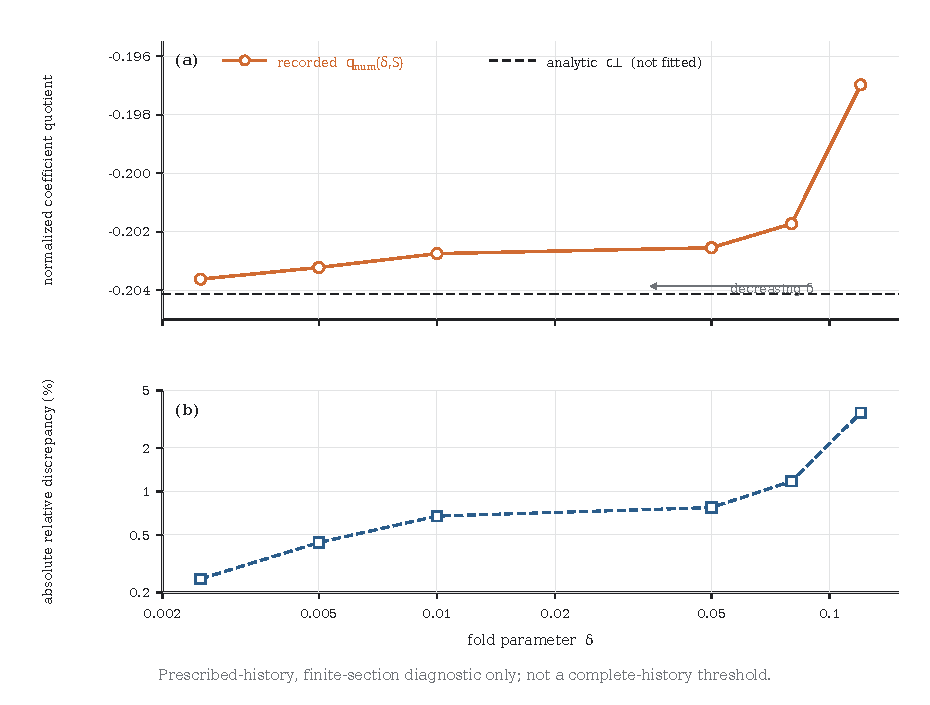
\includegraphics[width=.82\textwidth]{figures/figure2_threshold_convergence.pdf}
\caption{Numerical diagnostic for \cref{eq:numerical-quotient}.  The
normalized central quotient approaches the analytic coefficient
\cref{eq:numerical-target} along a sequence with decreasing \(\del\) and
increasing finite section \(S\).  The lower panel reports relative
discrepancy.  This plot checks sign and scale; it is not used in the proof.}
\label{fig:numerical-convergence}
\end{figure}

\FloatBarrier

The distinction matters.  The theorem constructs both one-sided traces on
the parameter-dependent history graph and equates their complete histories.
The diagnostic instead supplies one incoming history and asks for a scalar
outgoing energy.  It can therefore falsify a sign or normalization error in
\cref{eq:transverse-return-coefficient}, but convergence of
\cref{eq:numerical-quotient} cannot prove preparation independence,
section independence, or the uniform remainder in \cref{eq:main-law}.
Full-precision data, solver tolerances, step refinements, source hashes, and
the reproduction command are included with the supplementary code.
